\documentclass[twoside]{book}

% Packages required by doxygen
\usepackage{fixltx2e}
\usepackage{calc}
\usepackage{doxygen}
\usepackage[export]{adjustbox} % also loads graphicx
\usepackage{graphicx}
\usepackage[utf8]{inputenc}
\usepackage{makeidx}
\usepackage{multicol}
\usepackage{multirow}
\PassOptionsToPackage{warn}{textcomp}
\usepackage{textcomp}
\usepackage[nointegrals]{wasysym}
\usepackage[table]{xcolor}

% Font selection
\usepackage[T1]{fontenc}
\usepackage[scaled=.90]{helvet}
\usepackage{courier}
\usepackage{amssymb}
\usepackage{sectsty}
\renewcommand{\familydefault}{\sfdefault}
\allsectionsfont{%
  \fontseries{bc}\selectfont%
  \color{darkgray}%
}
\renewcommand{\DoxyLabelFont}{%
  \fontseries{bc}\selectfont%
  \color{darkgray}%
}
\newcommand{\+}{\discretionary{\mbox{\scriptsize$\hookleftarrow$}}{}{}}

% Page & text layout
\usepackage{geometry}
\geometry{%
  a4paper,%
  top=2.5cm,%
  bottom=2.5cm,%
  left=2.5cm,%
  right=2.5cm%
}
\tolerance=750
\hfuzz=15pt
\hbadness=750
\setlength{\emergencystretch}{15pt}
\setlength{\parindent}{0cm}
\setlength{\parskip}{3ex plus 2ex minus 2ex}
\makeatletter
\renewcommand{\paragraph}{%
  \@startsection{paragraph}{4}{0ex}{-1.0ex}{1.0ex}{%
    \normalfont\normalsize\bfseries\SS@parafont%
  }%
}
\renewcommand{\subparagraph}{%
  \@startsection{subparagraph}{5}{0ex}{-1.0ex}{1.0ex}{%
    \normalfont\normalsize\bfseries\SS@subparafont%
  }%
}
\makeatother

% Headers & footers
\usepackage{fancyhdr}
\pagestyle{fancyplain}
\fancyhead[LE]{\fancyplain{}{\bfseries\thepage}}
\fancyhead[CE]{\fancyplain{}{}}
\fancyhead[RE]{\fancyplain{}{\bfseries\leftmark}}
\fancyhead[LO]{\fancyplain{}{\bfseries\rightmark}}
\fancyhead[CO]{\fancyplain{}{}}
\fancyhead[RO]{\fancyplain{}{\bfseries\thepage}}
\fancyfoot[LE]{\fancyplain{}{}}
\fancyfoot[CE]{\fancyplain{}{}}
\fancyfoot[RE]{\fancyplain{}{\bfseries\scriptsize Generated by Doxygen }}
\fancyfoot[LO]{\fancyplain{}{\bfseries\scriptsize Generated by Doxygen }}
\fancyfoot[CO]{\fancyplain{}{}}
\fancyfoot[RO]{\fancyplain{}{}}
\renewcommand{\footrulewidth}{0.4pt}
\renewcommand{\chaptermark}[1]{%
  \markboth{#1}{}%
}
\renewcommand{\sectionmark}[1]{%
  \markright{\thesection\ #1}%
}

% Indices & bibliography
\usepackage{natbib}
\usepackage[titles]{tocloft}
\setcounter{tocdepth}{3}
\setcounter{secnumdepth}{5}
\makeindex

% Hyperlinks (required, but should be loaded last)
\usepackage{ifpdf}
\ifpdf
  \usepackage[pdftex,pagebackref=true]{hyperref}
\else
  \usepackage[ps2pdf,pagebackref=true]{hyperref}
\fi
\hypersetup{%
  colorlinks=true,%
  linkcolor=blue,%
  citecolor=blue,%
  unicode%
}

% Custom commands
\newcommand{\clearemptydoublepage}{%
  \newpage{\pagestyle{empty}\cleardoublepage}%
}

\usepackage{caption}
\captionsetup{labelsep=space,justification=centering,font={bf},singlelinecheck=off,skip=4pt,position=top}

%===== C O N T E N T S =====

\begin{document}

% Titlepage & ToC
\hypersetup{pageanchor=false,
             bookmarksnumbered=true,
             pdfencoding=unicode
            }
\pagenumbering{alph}
\begin{titlepage}
\vspace*{7cm}
\begin{center}%
{\Large Correction Texte Chat }\\
\vspace*{1cm}
{\large Generated by Doxygen 1.8.13}\\
\end{center}
\end{titlepage}
\clearemptydoublepage
\pagenumbering{roman}
\tableofcontents
\clearemptydoublepage
\pagenumbering{arabic}
\hypersetup{pageanchor=true}

%--- Begin generated contents ---
\chapter{Hierarchical Index}
\section{Class Hierarchy}
This inheritance list is sorted roughly, but not completely, alphabetically\+:\begin{DoxyCompactList}
\item \contentsline{section}{Atomic\+Float}{\pageref{classAtomicFloat}}{}
\item \contentsline{section}{Database}{\pageref{classDatabase}}{}
\item \contentsline{section}{Executor$<$ Return\+Type, Arg\+Type $>$}{\pageref{classExecutor}}{}
\item \contentsline{section}{Executor$<$ void, void $>$}{\pageref{classExecutor_3_01void_00_01void_01_4}}{}
\item \contentsline{section}{File}{\pageref{classFile}}{}
\item \contentsline{section}{Gram}{\pageref{classGram}}{}
\item \contentsline{section}{Grams\+Counter}{\pageref{classGramsCounter}}{}
\item \contentsline{section}{std\+:\+:hash$<$ Gram $>$}{\pageref{structstd_1_1hash_3_01Gram_01_4}}{}
\item \contentsline{section}{Layout}{\pageref{classLayout}}{}
\item \contentsline{section}{Lexicon}{\pageref{classLexicon}}{}
\item \contentsline{section}{Tokenizer}{\pageref{classTokenizer}}{}
\item \contentsline{section}{Viterbi}{\pageref{classViterbi}}{}
\item \contentsline{section}{Word\+Translations}{\pageref{classWordTranslations}}{}
\item \contentsline{section}{Word\+Translator}{\pageref{classWordTranslator}}{}
\begin{DoxyCompactList}
\item \contentsline{section}{Levenshtein\+Translator}{\pageref{classLevenshteinTranslator}}{}
\item \contentsline{section}{Translation\+Table}{\pageref{classTranslationTable}}{}
\end{DoxyCompactList}
\end{DoxyCompactList}

\chapter{Class Index}
\section{Class List}
Here are the classes, structs, unions and interfaces with brief descriptions\+:\begin{DoxyCompactList}
\item\contentsline{section}{\hyperlink{classAtomicFloat}{Atomic\+Float} }{\pageref{classAtomicFloat}}{}
\item\contentsline{section}{\hyperlink{classDatabase}{Database} \\*Contains necessary data to perform a correction }{\pageref{classDatabase}}{}
\item\contentsline{section}{\hyperlink{classExecutor}{Executor$<$ Return\+Type, Arg\+Type $>$} }{\pageref{classExecutor}}{}
\item\contentsline{section}{\hyperlink{classExecutor_3_01void_00_01void_01_4}{Executor$<$ void, void $>$} }{\pageref{classExecutor_3_01void_00_01void_01_4}}{}
\item\contentsline{section}{\hyperlink{classFile}{File} }{\pageref{classFile}}{}
\item\contentsline{section}{\hyperlink{classGram}{Gram} }{\pageref{classGram}}{}
\item\contentsline{section}{\hyperlink{classGramsCounter}{Grams\+Counter} }{\pageref{classGramsCounter}}{}
\item\contentsline{section}{\hyperlink{structstd_1_1hash_3_01Gram_01_4}{std\+::hash$<$ Gram $>$} }{\pageref{structstd_1_1hash_3_01Gram_01_4}}{}
\item\contentsline{section}{\hyperlink{classLayout}{Layout} }{\pageref{classLayout}}{}
\item\contentsline{section}{\hyperlink{classLevenshteinTranslator}{Levenshtein\+Translator} }{\pageref{classLevenshteinTranslator}}{}
\item\contentsline{section}{\hyperlink{classLexicon}{Lexicon} }{\pageref{classLexicon}}{}
\item\contentsline{section}{\hyperlink{classTokenizer}{Tokenizer} }{\pageref{classTokenizer}}{}
\item\contentsline{section}{\hyperlink{classTranslationTable}{Translation\+Table} }{\pageref{classTranslationTable}}{}
\item\contentsline{section}{\hyperlink{classViterbi}{Viterbi} }{\pageref{classViterbi}}{}
\item\contentsline{section}{\hyperlink{classWordTranslations}{Word\+Translations} }{\pageref{classWordTranslations}}{}
\item\contentsline{section}{\hyperlink{classWordTranslator}{Word\+Translator} }{\pageref{classWordTranslator}}{}
\end{DoxyCompactList}

\chapter{File Index}
\section{File List}
Here is a list of all documented files with brief descriptions\+:\begin{DoxyCompactList}
\item\contentsline{section}{{\bfseries Atomic\+Float.\+hpp} }{\pageref{AtomicFloat_8hpp}}{}
\item\contentsline{section}{{\bfseries colors.\+hpp} }{\pageref{colors_8hpp}}{}
\item\contentsline{section}{\hyperlink{Database_8hpp}{Database.\+hpp} }{\pageref{Database_8hpp}}{}
\item\contentsline{section}{{\bfseries Executor.\+hpp} }{\pageref{Executor_8hpp}}{}
\item\contentsline{section}{{\bfseries File.\+hpp} }{\pageref{File_8hpp}}{}
\item\contentsline{section}{{\bfseries Grams\+Counter.\+hpp} }{\pageref{GramsCounter_8hpp}}{}
\item\contentsline{section}{{\bfseries Layout.\+hpp} }{\pageref{Layout_8hpp}}{}
\item\contentsline{section}{{\bfseries Levenshtein\+Translator.\+hpp} }{\pageref{LevenshteinTranslator_8hpp}}{}
\item\contentsline{section}{{\bfseries Lexicon.\+hpp} }{\pageref{Lexicon_8hpp}}{}
\item\contentsline{section}{{\bfseries Tokenizer.\+hpp} }{\pageref{Tokenizer_8hpp}}{}
\item\contentsline{section}{{\bfseries Translation\+Table.\+hpp} }{\pageref{TranslationTable_8hpp}}{}
\item\contentsline{section}{{\bfseries util.\+hpp} }{\pageref{util_8hpp}}{}
\item\contentsline{section}{{\bfseries Viterbi.\+hpp} }{\pageref{Viterbi_8hpp}}{}
\item\contentsline{section}{{\bfseries Word\+Translator.\+hpp} }{\pageref{WordTranslator_8hpp}}{}
\end{DoxyCompactList}

\chapter{Class Documentation}
\hypertarget{classAtomicFloat}{}\section{Atomic\+Float Class Reference}
\label{classAtomicFloat}\index{Atomic\+Float@{Atomic\+Float}}
\subsection*{Public Member Functions}
\begin{DoxyCompactItemize}
\item 
\mbox{\Hypertarget{classAtomicFloat_af11cff090e6c3e37996efe67157a9301}\label{classAtomicFloat_af11cff090e6c3e37996efe67157a9301}} 
{\bfseries Atomic\+Float} (float value=0.\+0f)
\item 
\mbox{\Hypertarget{classAtomicFloat_a0346bea59f0fd4f4876e4c76dc5783f5}\label{classAtomicFloat_a0346bea59f0fd4f4876e4c76dc5783f5}} 
{\bfseries Atomic\+Float} (const \hyperlink{classAtomicFloat}{Atomic\+Float} \&model)
\item 
\mbox{\Hypertarget{classAtomicFloat_a396866e22a2a7cd5b9c49149f4014df3}\label{classAtomicFloat_a396866e22a2a7cd5b9c49149f4014df3}} 
{\bfseries operator float} () const
\item 
\mbox{\Hypertarget{classAtomicFloat_a38d6e55da00fa162185fc2bfaef16239}\label{classAtomicFloat_a38d6e55da00fa162185fc2bfaef16239}} 
float {\bfseries load} () const
\item 
\mbox{\Hypertarget{classAtomicFloat_a55fb3f675d4c44e80998b228cce112ce}\label{classAtomicFloat_a55fb3f675d4c44e80998b228cce112ce}} 
\hyperlink{classAtomicFloat}{Atomic\+Float} \& {\bfseries operator+=} (float increment)
\item 
\mbox{\Hypertarget{classAtomicFloat_aa913c328fe196661d56406bc1902fa2b}\label{classAtomicFloat_aa913c328fe196661d56406bc1902fa2b}} 
\hyperlink{classAtomicFloat}{Atomic\+Float} \& {\bfseries operator=} (float value)
\item 
\mbox{\Hypertarget{classAtomicFloat_abe03f0bf79b3f0eebcfec3110dfa0cd1}\label{classAtomicFloat_abe03f0bf79b3f0eebcfec3110dfa0cd1}} 
\hyperlink{classAtomicFloat}{Atomic\+Float} \& {\bfseries operator=} (const \hyperlink{classAtomicFloat}{Atomic\+Float} \&model)
\end{DoxyCompactItemize}
\subsection*{Static Public Member Functions}
\begin{DoxyCompactItemize}
\item 
\mbox{\Hypertarget{classAtomicFloat_ab842d3b53d55a84deac19875cb861cf2}\label{classAtomicFloat_ab842d3b53d55a84deac19875cb861cf2}} 
static constexpr long long int {\bfseries scale} (float f)
\end{DoxyCompactItemize}
\subsection*{Static Public Attributes}
\begin{DoxyCompactItemize}
\item 
\mbox{\Hypertarget{classAtomicFloat_a1070b6e6618d84e7008f3a87d229420d}\label{classAtomicFloat_a1070b6e6618d84e7008f3a87d229420d}} 
static constexpr float {\bfseries scaling} = 1000 $\ast$ 1000
\end{DoxyCompactItemize}


The documentation for this class was generated from the following files\+:\begin{DoxyCompactItemize}
\item 
Atomic\+Float.\+hpp\item 
Atomic\+Float.\+cpp\end{DoxyCompactItemize}

\hypertarget{classDatabase}{}\section{Database Class Reference}
\label{classDatabase}\index{Database@{Database}}


Contains necessary data to perform a correction.  




{\ttfamily \#include $<$Database.\+hpp$>$}

\subsection*{Public Member Functions}
\begin{DoxyCompactItemize}
\item 
\hyperlink{classDatabase_a4703c80e6969d33565ea340f768fdadf}{Database} ()
\begin{DoxyCompactList}\small\item\em Constructor. \end{DoxyCompactList}\item 
void \hyperlink{classDatabase_a98b7974dc1e1b76456fa35cc2665e6f9}{build\+From\+Corpus} (std\+::string correct\+Name, std\+::string incorrect\+Name)
\begin{DoxyCompactList}\small\item\em Build the \hyperlink{classDatabase}{Database}, long process. \end{DoxyCompactList}\item 
void \hyperlink{classDatabase_a3dbadcd3a09ae36cb36c73519e34b328}{read\+From\+Files} (std\+::string incorrect\+Filename, std\+::string correct\+Filename, std\+::string grams\+Filename, std\+::string table\+Filename)
\begin{DoxyCompactList}\small\item\em Read the \hyperlink{classDatabase}{Database} from files created by build\+From\+Corpus. \end{DoxyCompactList}\end{DoxyCompactItemize}
\subsection*{Public Attributes}
\begin{DoxyCompactItemize}
\item 
\mbox{\Hypertarget{classDatabase_affb4d666b7bac4f76aca3863e158cf11}\label{classDatabase_affb4d666b7bac4f76aca3863e158cf11}} 
friend {\bfseries Viterbi}
\end{DoxyCompactItemize}


\subsection{Detailed Description}
Contains necessary data to perform a correction. 

Creation of the \hyperlink{classDatabase}{Database} is a long process, that is why you only need to build it once. During the build process several files representing the \hyperlink{classDatabase}{Database} will be written. \hyperlink{classDatabase}{Database} can then be directly loaded from those files. 

\subsection{Constructor \& Destructor Documentation}
\mbox{\Hypertarget{classDatabase_a4703c80e6969d33565ea340f768fdadf}\label{classDatabase_a4703c80e6969d33565ea340f768fdadf}} 
\index{Database@{Database}!Database@{Database}}
\index{Database@{Database}!Database@{Database}}
\subsubsection{\texorpdfstring{Database()}{Database()}}
{\footnotesize\ttfamily Database\+::\+Database (\begin{DoxyParamCaption}{ }\end{DoxyParamCaption})}



Constructor. 

When constructed the \hyperlink{classDatabase}{Database} represents nothing and must not be used as it is. You have to call build\+From\+Corpus or read\+From\+Files in order to initialize it. 

\subsection{Member Function Documentation}
\mbox{\Hypertarget{classDatabase_a98b7974dc1e1b76456fa35cc2665e6f9}\label{classDatabase_a98b7974dc1e1b76456fa35cc2665e6f9}} 
\index{Database@{Database}!build\+From\+Corpus@{build\+From\+Corpus}}
\index{build\+From\+Corpus@{build\+From\+Corpus}!Database@{Database}}
\subsubsection{\texorpdfstring{build\+From\+Corpus()}{buildFromCorpus()}}
{\footnotesize\ttfamily void Database\+::build\+From\+Corpus (\begin{DoxyParamCaption}\item[{std\+::string}]{correct\+Name,  }\item[{std\+::string}]{incorrect\+Name }\end{DoxyParamCaption})}



Build the \hyperlink{classDatabase}{Database}, long process. 

Construct \hyperlink{classLexicon}{Lexicon}, \hyperlink{classGramsCounter}{Grams\+Counter}, \hyperlink{classTranslationTable}{Translation\+Table} using the files passed as parameters. Creates a number of files, that can later be used for read\+From\+Files.


\begin{DoxyParams}{Parameters}
{\em correct\+Name} & Path to the file containing the corrected corpus. \\
\hline
{\em incorrect\+Name} & Path to the file containing the un-\/corrected corpus. \\
\hline
\end{DoxyParams}
\mbox{\Hypertarget{classDatabase_a3dbadcd3a09ae36cb36c73519e34b328}\label{classDatabase_a3dbadcd3a09ae36cb36c73519e34b328}} 
\index{Database@{Database}!read\+From\+Files@{read\+From\+Files}}
\index{read\+From\+Files@{read\+From\+Files}!Database@{Database}}
\subsubsection{\texorpdfstring{read\+From\+Files()}{readFromFiles()}}
{\footnotesize\ttfamily void Database\+::read\+From\+Files (\begin{DoxyParamCaption}\item[{std\+::string}]{incorrect\+Filename,  }\item[{std\+::string}]{correct\+Filename,  }\item[{std\+::string}]{grams\+Filename,  }\item[{std\+::string}]{table\+Filename }\end{DoxyParamCaption})}



Read the \hyperlink{classDatabase}{Database} from files created by build\+From\+Corpus. 


\begin{DoxyParams}{Parameters}
{\em incorrect\+Filename} & Path to the file containing \hyperlink{classLexicon}{Lexicon} incorrect\+Lexicon. \\
\hline
{\em correct\+Filename} & Path to the file containing \hyperlink{classLexicon}{Lexicon} correct\+Lexicon. \\
\hline
{\em grams\+Filename} & Path to the file containing the \hyperlink{classGramsCounter}{Grams\+Counter}. \\
\hline
{\em table\+Filename} & Path to the file containing the \hyperlink{classTranslationTable}{Translation\+Table}. \\
\hline
\end{DoxyParams}


The documentation for this class was generated from the following files\+:\begin{DoxyCompactItemize}
\item 
\hyperlink{Database_8hpp}{Database.\+hpp}\item 
Database.\+cpp\end{DoxyCompactItemize}

\hypertarget{classExecutor}{}\section{Executor$<$ Return\+Type, Arg\+Type $>$ Class Template Reference}
\label{classExecutor}\index{Executor$<$ Return\+Type, Arg\+Type $>$@{Executor$<$ Return\+Type, Arg\+Type $>$}}
\subsection*{Public Member Functions}
\begin{DoxyCompactItemize}
\item 
\mbox{\Hypertarget{classExecutor_a783d0d5754142c9e56e0c0a4145d44ce}\label{classExecutor_a783d0d5754142c9e56e0c0a4145d44ce}} 
{\bfseries Executor} (int nb\+Threads=std\+::thread\+::hardware\+\_\+concurrency())
\item 
\mbox{\Hypertarget{classExecutor_a04ca3995fd6dccf42d235d9695ec0903}\label{classExecutor_a04ca3995fd6dccf42d235d9695ec0903}} 
void {\bfseries add\+Task} (std\+::function$<$ Return\+Type(Arg\+Type)$>$ func, Arg\+Type argument)
\item 
\mbox{\Hypertarget{classExecutor_a5905222a566b53ea585f83ea8fd1e565}\label{classExecutor_a5905222a566b53ea585f83ea8fd1e565}} 
void {\bfseries run} ()
\item 
\mbox{\Hypertarget{classExecutor_a3e13df6ead70066b3b26c3e83233e9e6}\label{classExecutor_a3e13df6ead70066b3b26c3e83233e9e6}} 
void {\bfseries clear} ()
\end{DoxyCompactItemize}


The documentation for this class was generated from the following file\+:\begin{DoxyCompactItemize}
\item 
Executor.\+hpp\end{DoxyCompactItemize}

\hypertarget{classExecutor_3_01void_00_01void_01_4}{}\section{Executor$<$ void, void $>$ Class Template Reference}
\label{classExecutor_3_01void_00_01void_01_4}\index{Executor$<$ void, void $>$@{Executor$<$ void, void $>$}}
\subsection*{Public Member Functions}
\begin{DoxyCompactItemize}
\item 
\mbox{\Hypertarget{classExecutor_3_01void_00_01void_01_4_a1f924354573e9debd3cc97ff2378bb3b}\label{classExecutor_3_01void_00_01void_01_4_a1f924354573e9debd3cc97ff2378bb3b}} 
{\bfseries Executor} (int nb\+Threads=std\+::thread\+::hardware\+\_\+concurrency())
\item 
\mbox{\Hypertarget{classExecutor_3_01void_00_01void_01_4_afdc61e42ff31fb4a18562cf4d3d5e0b3}\label{classExecutor_3_01void_00_01void_01_4_afdc61e42ff31fb4a18562cf4d3d5e0b3}} 
void {\bfseries add\+Task} (std\+::function$<$ void(void)$>$ func)
\item 
\mbox{\Hypertarget{classExecutor_3_01void_00_01void_01_4_aba601150cd9b408bf858f4ad15b64ed4}\label{classExecutor_3_01void_00_01void_01_4_aba601150cd9b408bf858f4ad15b64ed4}} 
void {\bfseries run} ()
\item 
\mbox{\Hypertarget{classExecutor_3_01void_00_01void_01_4_ac1ae73ad5bdca1a0a71084bfef74e016}\label{classExecutor_3_01void_00_01void_01_4_ac1ae73ad5bdca1a0a71084bfef74e016}} 
void {\bfseries clear} ()
\end{DoxyCompactItemize}


The documentation for this class was generated from the following file\+:\begin{DoxyCompactItemize}
\item 
Executor.\+hpp\end{DoxyCompactItemize}

\hypertarget{classFile}{}\section{File Class Reference}
\label{classFile}\index{File@{File}}
\subsection*{Public Member Functions}
\begin{DoxyCompactItemize}
\item 
\mbox{\Hypertarget{classFile_a8574f47a4eff4fc44bd60919c61610d3}\label{classFile_a8574f47a4eff4fc44bd60919c61610d3}} 
{\bfseries File} (const std\+::string \&filename, const std\+::string \&mode)
\item 
\mbox{\Hypertarget{classFile_a60b843d95156968bb69e26e9171b2c57}\label{classFile_a60b843d95156968bb69e26e9171b2c57}} 
char {\bfseries peek} ()
\item 
\mbox{\Hypertarget{classFile_a93457cfa8895f0eb185f4b47d3f36fd9}\label{classFile_a93457cfa8895f0eb185f4b47d3f36fd9}} 
bool {\bfseries is\+Finished} ()
\item 
\mbox{\Hypertarget{classFile_a9377d79b66b40cef676db07e67871ca8}\label{classFile_a9377d79b66b40cef676db07e67871ca8}} 
char {\bfseries get\+Char} ()
\item 
\mbox{\Hypertarget{classFile_aad8d72b0d1ebd8f10f6b031065c9271e}\label{classFile_aad8d72b0d1ebd8f10f6b031065c9271e}} 
void {\bfseries unget\+Char} (char c)
\item 
\mbox{\Hypertarget{classFile_aa538ff162143bbfe6782b9ebe33426b4}\label{classFile_aa538ff162143bbfe6782b9ebe33426b4}} 
F\+I\+LE $\ast$ {\bfseries get\+Descriptor} ()
\item 
\mbox{\Hypertarget{classFile_ac6d74a81bad59ad73501c3b89280b7e3}\label{classFile_ac6d74a81bad59ad73501c3b89280b7e3}} 
const std\+::string \& {\bfseries get\+Name} ()
\item 
\mbox{\Hypertarget{classFile_a86532a7e52e5c6a75ec98b3c46f77376}\label{classFile_a86532a7e52e5c6a75ec98b3c46f77376}} 
char {\bfseries read\+Until} (char c)
\item 
\mbox{\Hypertarget{classFile_ad5878720bf6a72548ec8f2fa5598ed45}\label{classFile_ad5878720bf6a72548ec8f2fa5598ed45}} 
char {\bfseries read\+Until} (const std\+::function$<$ bool(char)$>$ \&condition)
\item 
\mbox{\Hypertarget{classFile_a80c6611e0e9e89f45307f7606e643cfa}\label{classFile_a80c6611e0e9e89f45307f7606e643cfa}} 
void {\bfseries rewind} ()
\end{DoxyCompactItemize}


The documentation for this class was generated from the following files\+:\begin{DoxyCompactItemize}
\item 
File.\+hpp\item 
File.\+cpp\end{DoxyCompactItemize}

\hypertarget{classGram}{}\section{Gram Class Reference}
\label{classGram}\index{Gram@{Gram}}
\subsection*{Public Member Functions}
\begin{DoxyCompactItemize}
\item 
\mbox{\Hypertarget{classGram_a03b03e2ae7a911ae18da92336720a2f6}\label{classGram_a03b03e2ae7a911ae18da92336720a2f6}} 
bool {\bfseries operator==} (const \hyperlink{classGram}{Gram} \&other) const
\end{DoxyCompactItemize}
\subsection*{Friends}
\begin{DoxyCompactItemize}
\item 
\mbox{\Hypertarget{classGram_a7448f2740fc0d47d2dc39bb494954eed}\label{classGram_a7448f2740fc0d47d2dc39bb494954eed}} 
class {\bfseries std\+::hash$<$ Gram $>$}
\item 
\mbox{\Hypertarget{classGram_a82d274cb5114ab32759b80802e86048b}\label{classGram_a82d274cb5114ab32759b80802e86048b}} 
class {\bfseries Grams\+Counter}
\end{DoxyCompactItemize}


The documentation for this class was generated from the following files\+:\begin{DoxyCompactItemize}
\item 
Grams\+Counter.\+hpp\item 
Grams\+Counter.\+cpp\end{DoxyCompactItemize}

\hypertarget{classGramsCounter}{}\section{Grams\+Counter Class Reference}
\label{classGramsCounter}\index{Grams\+Counter@{Grams\+Counter}}
\subsection*{Public Member Functions}
\begin{DoxyCompactItemize}
\item 
\mbox{\Hypertarget{classGramsCounter_aedbfec5dc4db03ac98f3f28362f124a2}\label{classGramsCounter_aedbfec5dc4db03ac98f3f28362f124a2}} 
void {\bfseries add\+Gram} (unsigned int t1)
\item 
\mbox{\Hypertarget{classGramsCounter_af65dc5d8a469ed925a7b23dce0429c1c}\label{classGramsCounter_af65dc5d8a469ed925a7b23dce0429c1c}} 
void {\bfseries add\+Gram} (unsigned int t1, unsigned int t2)
\item 
\mbox{\Hypertarget{classGramsCounter_a7fa78eccbb6b347f2198545b51cbdd1e}\label{classGramsCounter_a7fa78eccbb6b347f2198545b51cbdd1e}} 
void {\bfseries add\+Gram} (unsigned int t1, unsigned int t2, unsigned int t3)
\item 
\mbox{\Hypertarget{classGramsCounter_a532728e0311b5f5cdd0dd9f2cd0b5115}\label{classGramsCounter_a532728e0311b5f5cdd0dd9f2cd0b5115}} 
float {\bfseries get\+Prob} (unsigned int t1) const
\item 
\mbox{\Hypertarget{classGramsCounter_ad9cf8f02d0a2cabcd17cac6c945b3ef6}\label{classGramsCounter_ad9cf8f02d0a2cabcd17cac6c945b3ef6}} 
float {\bfseries get\+Prob} (unsigned int t1, unsigned int t2) const
\item 
\mbox{\Hypertarget{classGramsCounter_aaf9e73b2f78e2e062bac7fd3892bdf62}\label{classGramsCounter_aaf9e73b2f78e2e062bac7fd3892bdf62}} 
float {\bfseries get\+Prob} (unsigned int t1, unsigned int t2, unsigned int t3) const
\item 
\mbox{\Hypertarget{classGramsCounter_ab6e4e5ed53e00ba86deb737e84f46372}\label{classGramsCounter_ab6e4e5ed53e00ba86deb737e84f46372}} 
float {\bfseries get\+Log\+Prob} (unsigned int t1) const
\item 
\mbox{\Hypertarget{classGramsCounter_aac64cb91593a3d4b15d6821e73cfa476}\label{classGramsCounter_aac64cb91593a3d4b15d6821e73cfa476}} 
float {\bfseries get\+Log\+Prob} (unsigned int t1, unsigned int t2) const
\item 
\mbox{\Hypertarget{classGramsCounter_a714193c3fb467239794fe183befff6fc}\label{classGramsCounter_a714193c3fb467239794fe183befff6fc}} 
float {\bfseries get\+Log\+Prob} (unsigned int t1, unsigned int t2, unsigned int t3) const
\item 
\mbox{\Hypertarget{classGramsCounter_a8019ed3baf4bbf6d432177ba971095fc}\label{classGramsCounter_a8019ed3baf4bbf6d432177ba971095fc}} 
void {\bfseries read} (\hyperlink{classFile}{File} \&input)
\item 
\mbox{\Hypertarget{classGramsCounter_a05ccff4ad467e1200e2e202e572bb2ca}\label{classGramsCounter_a05ccff4ad467e1200e2e202e572bb2ca}} 
void {\bfseries print} (F\+I\+LE $\ast$output)
\item 
\mbox{\Hypertarget{classGramsCounter_a1c70211f6f1c5a81bd1711f6909d914b}\label{classGramsCounter_a1c70211f6f1c5a81bd1711f6909d914b}} 
void {\bfseries print} (F\+I\+LE $\ast$output, \hyperlink{classLexicon}{Lexicon} \&lexicon)
\end{DoxyCompactItemize}


The documentation for this class was generated from the following files\+:\begin{DoxyCompactItemize}
\item 
Grams\+Counter.\+hpp\item 
Grams\+Counter.\+cpp\end{DoxyCompactItemize}

\hypertarget{structstd_1_1hash_3_01Gram_01_4}{}\section{std\+:\+:hash$<$ Gram $>$ Struct Template Reference}
\label{structstd_1_1hash_3_01Gram_01_4}\index{std\+::hash$<$ Gram $>$@{std\+::hash$<$ Gram $>$}}
\subsection*{Public Member Functions}
\begin{DoxyCompactItemize}
\item 
\mbox{\Hypertarget{structstd_1_1hash_3_01Gram_01_4_ad947fc278a6bcbee417f5426ca01eaaf}\label{structstd_1_1hash_3_01Gram_01_4_ad947fc278a6bcbee417f5426ca01eaaf}} 
size\+\_\+t {\bfseries operator()} (const \hyperlink{classGram}{Gram} \&g) const
\end{DoxyCompactItemize}


The documentation for this struct was generated from the following file\+:\begin{DoxyCompactItemize}
\item 
Grams\+Counter.\+hpp\end{DoxyCompactItemize}

\hypertarget{classLayout}{}\section{Layout Class Reference}
\label{classLayout}\index{Layout@{Layout}}
\subsection*{Public Member Functions}
\begin{DoxyCompactItemize}
\item 
\mbox{\Hypertarget{classLayout_a668390329ed1b47bb509773c5af6bab4}\label{classLayout_a668390329ed1b47bb509773c5af6bab4}} 
{\bfseries Layout} (\hyperlink{classFile}{File} $\ast$base\+Text, \hyperlink{classFile}{File} $\ast$corrected\+Text)
\item 
\mbox{\Hypertarget{classLayout_a3b4a785ff44fa3c68a06a5ba21fe8a3a}\label{classLayout_a3b4a785ff44fa3c68a06a5ba21fe8a3a}} 
void {\bfseries transfer\+Layout} (\hyperlink{classFile}{File} $\ast$target)
\end{DoxyCompactItemize}


The documentation for this class was generated from the following files\+:\begin{DoxyCompactItemize}
\item 
Layout.\+hpp\item 
Layout.\+cpp\end{DoxyCompactItemize}

\hypertarget{classLevenshteinTranslator}{}\section{Levenshtein\+Translator Class Reference}
\label{classLevenshteinTranslator}\index{Levenshtein\+Translator@{Levenshtein\+Translator}}
Inheritance diagram for Levenshtein\+Translator\+:\begin{figure}[H]
\begin{center}
\leavevmode
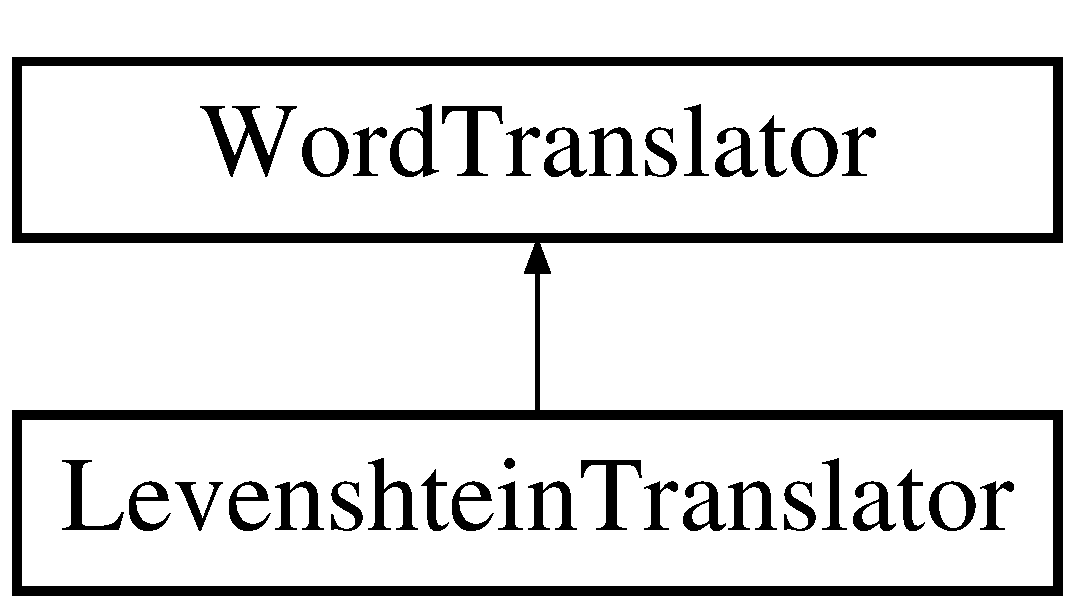
\includegraphics[height=2.000000cm]{classLevenshteinTranslator}
\end{center}
\end{figure}
\subsection*{Public Member Functions}
\begin{DoxyCompactItemize}
\item 
\mbox{\Hypertarget{classLevenshteinTranslator_a549cbb265018570510b836e2cc5c8128}\label{classLevenshteinTranslator_a549cbb265018570510b836e2cc5c8128}} 
{\bfseries Levenshtein\+Translator} (\hyperlink{classLexicon}{Lexicon} \&correct\+Lexicon, \hyperlink{classLexicon}{Lexicon} \&incorrect\+Lexicon)
\item 
\mbox{\Hypertarget{classLevenshteinTranslator_af78505539527d0678ca35d9cb63910d4}\label{classLevenshteinTranslator_af78505539527d0678ca35d9cb63910d4}} 
void {\bfseries add\+Translations} (\hyperlink{classWordTranslations}{Word\+Translations} \&actual)
\end{DoxyCompactItemize}
\subsection*{Additional Inherited Members}


The documentation for this class was generated from the following files\+:\begin{DoxyCompactItemize}
\item 
Levenshtein\+Translator.\+hpp\item 
Levenshtein\+Translator.\+cpp\end{DoxyCompactItemize}

\hypertarget{classLexicon}{}\section{Lexicon Class Reference}
\label{classLexicon}\index{Lexicon@{Lexicon}}
\subsection*{Public Member Functions}
\begin{DoxyCompactItemize}
\item 
\mbox{\Hypertarget{classLexicon_ab98081cb72cada5ba51138752d81d898}\label{classLexicon_ab98081cb72cada5ba51138752d81d898}} 
void {\bfseries init\+Maps} (std\+::unordered\+\_\+map$<$ std\+::string, unsigned int $>$ \&specials)
\item 
\mbox{\Hypertarget{classLexicon_a97daf7fd0ec322c4a64c94207467d9f0}\label{classLexicon_a97daf7fd0ec322c4a64c94207467d9f0}} 
unsigned int {\bfseries get\+Token} (std\+::string \&s)
\item 
\mbox{\Hypertarget{classLexicon_a7a286b953dc921e936d07ba514e929fe}\label{classLexicon_a7a286b953dc921e936d07ba514e929fe}} 
const std\+::unordered\+\_\+map$<$ std\+::string, unsigned int $>$ \& {\bfseries get\+Tokens} ()
\item 
\mbox{\Hypertarget{classLexicon_a328ff05786103c14ee4b0330829f3121}\label{classLexicon_a328ff05786103c14ee4b0330829f3121}} 
const std\+::string \& {\bfseries get\+String} (unsigned int token)
\item 
\mbox{\Hypertarget{classLexicon_a94b037e129bab580cdee396c8db8244c}\label{classLexicon_a94b037e129bab580cdee396c8db8244c}} 
unsigned int {\bfseries add\+Word} (const std\+::string \&word)
\item 
\mbox{\Hypertarget{classLexicon_a7126d888d4fceb8a58d21eb7ef95c2d6}\label{classLexicon_a7126d888d4fceb8a58d21eb7ef95c2d6}} 
void {\bfseries print} (F\+I\+LE $\ast$output)
\item 
\mbox{\Hypertarget{classLexicon_a7b3d53999b6e75aee8ffd2bb45ffdf70}\label{classLexicon_a7b3d53999b6e75aee8ffd2bb45ffdf70}} 
void {\bfseries read} (\hyperlink{classFile}{File} \&input)
\item 
\mbox{\Hypertarget{classLexicon_af4ed9570b9575341c43442150c1a748a}\label{classLexicon_af4ed9570b9575341c43442150c1a748a}} 
void {\bfseries copy} (const \hyperlink{classLexicon}{Lexicon} \&other)
\item 
\mbox{\Hypertarget{classLexicon_a25a9fff92015f05e2b315e31e74bee2f}\label{classLexicon_a25a9fff92015f05e2b315e31e74bee2f}} 
unsigned int {\bfseries get\+Max\+Token} () const
\end{DoxyCompactItemize}
\subsection*{Static Public Attributes}
\begin{DoxyCompactItemize}
\item 
\mbox{\Hypertarget{classLexicon_a59a48310a9dd34ca9dcd80d4ff047531}\label{classLexicon_a59a48310a9dd34ca9dcd80d4ff047531}} 
static constexpr unsigned int {\bfseries unknown} = 0
\item 
\mbox{\Hypertarget{classLexicon_a4c4bf4e37c916cccd9adaeb228429330}\label{classLexicon_a4c4bf4e37c916cccd9adaeb228429330}} 
static constexpr char {\bfseries unknown\+Str} \mbox{[}$\,$\mbox{]} = \char`\"{}U\+N\+K\+N\+O\+WN\char`\"{}
\item 
\mbox{\Hypertarget{classLexicon_a1dae4cf53e7c6343d3fe95d8754fee61}\label{classLexicon_a1dae4cf53e7c6343d3fe95d8754fee61}} 
static constexpr unsigned int {\bfseries mail} = 1
\item 
\mbox{\Hypertarget{classLexicon_a8e9965925b7ab956f4b0e6f82af4fcd8}\label{classLexicon_a8e9965925b7ab956f4b0e6f82af4fcd8}} 
static constexpr char {\bfseries mail\+Str} \mbox{[}$\,$\mbox{]} = \char`\"{}M\+A\+IL\char`\"{}
\item 
\mbox{\Hypertarget{classLexicon_a09c4d8bad7b44b9fce78f21aafd0e4d0}\label{classLexicon_a09c4d8bad7b44b9fce78f21aafd0e4d0}} 
static constexpr unsigned int {\bfseries number} = 2
\item 
\mbox{\Hypertarget{classLexicon_a39ff54ee2e7b5e6f523992ad92f30d6e}\label{classLexicon_a39ff54ee2e7b5e6f523992ad92f30d6e}} 
static constexpr char {\bfseries number\+Str} \mbox{[}$\,$\mbox{]} = \char`\"{}N\+U\+M\+B\+ER\char`\"{}
\item 
\mbox{\Hypertarget{classLexicon_ae796dbdb68e1a4758a9d40998bf40833}\label{classLexicon_ae796dbdb68e1a4758a9d40998bf40833}} 
static constexpr unsigned int {\bfseries proper\+Noun} = 3
\item 
\mbox{\Hypertarget{classLexicon_a9cf65fdf5226cc21152c3dd28c4a6fa4}\label{classLexicon_a9cf65fdf5226cc21152c3dd28c4a6fa4}} 
static constexpr char {\bfseries proper\+Noun\+Str} \mbox{[}$\,$\mbox{]} = \char`\"{}P\+R\+O\+P\+E\+R\+N\+O\+UN\char`\"{}
\item 
\mbox{\Hypertarget{classLexicon_a1e8cf6d17dea0480adbdb1f08f6c1167}\label{classLexicon_a1e8cf6d17dea0480adbdb1f08f6c1167}} 
static constexpr unsigned int {\bfseries date} = 4
\item 
\mbox{\Hypertarget{classLexicon_aa4457caaac6b659b7aeb8b40490a4438}\label{classLexicon_aa4457caaac6b659b7aeb8b40490a4438}} 
static constexpr char {\bfseries date\+Str} \mbox{[}$\,$\mbox{]} = \char`\"{}D\+A\+TE\char`\"{}
\end{DoxyCompactItemize}


The documentation for this class was generated from the following files\+:\begin{DoxyCompactItemize}
\item 
Lexicon.\+hpp\item 
Lexicon.\+cpp\end{DoxyCompactItemize}

\hypertarget{classTokenizer}{}\section{Tokenizer Class Reference}
\label{classTokenizer}\index{Tokenizer@{Tokenizer}}
\subsection*{Public Member Functions}
\begin{DoxyCompactItemize}
\item 
\mbox{\Hypertarget{classTokenizer_a82cea761b17a4a704faaab9531c3c501}\label{classTokenizer_a82cea761b17a4a704faaab9531c3c501}} 
{\bfseries Tokenizer} (\hyperlink{classLexicon}{Lexicon} \&lexicon)
\item 
\mbox{\Hypertarget{classTokenizer_af918888efe8c82cf983c13c675535859}\label{classTokenizer_af918888efe8c82cf983c13c675535859}} 
unsigned int {\bfseries tokenize} (\hyperlink{classFile}{File} \&corpus)
\item 
\mbox{\Hypertarget{classTokenizer_a9aaf23dcd5b05bebc558f78f7be99ea0}\label{classTokenizer_a9aaf23dcd5b05bebc558f78f7be99ea0}} 
\hyperlink{classFile}{File} $\ast$ {\bfseries tokenize} (\hyperlink{classFile}{File} \&corpus, const std\+::string \&path)
\end{DoxyCompactItemize}
\subsection*{Public Attributes}
\begin{DoxyCompactItemize}
\item 
\mbox{\Hypertarget{classTokenizer_a18b615fd0e04452cbc124a595ee5d372}\label{classTokenizer_a18b615fd0e04452cbc124a595ee5d372}} 
std\+::string {\bfseries word}
\end{DoxyCompactItemize}


The documentation for this class was generated from the following files\+:\begin{DoxyCompactItemize}
\item 
Tokenizer.\+hpp\item 
Tokenizer.\+cpp\end{DoxyCompactItemize}

\hypertarget{classTranslationTable}{}\section{Translation\+Table Class Reference}
\label{classTranslationTable}\index{Translation\+Table@{Translation\+Table}}
Inheritance diagram for Translation\+Table\+:\begin{figure}[H]
\begin{center}
\leavevmode
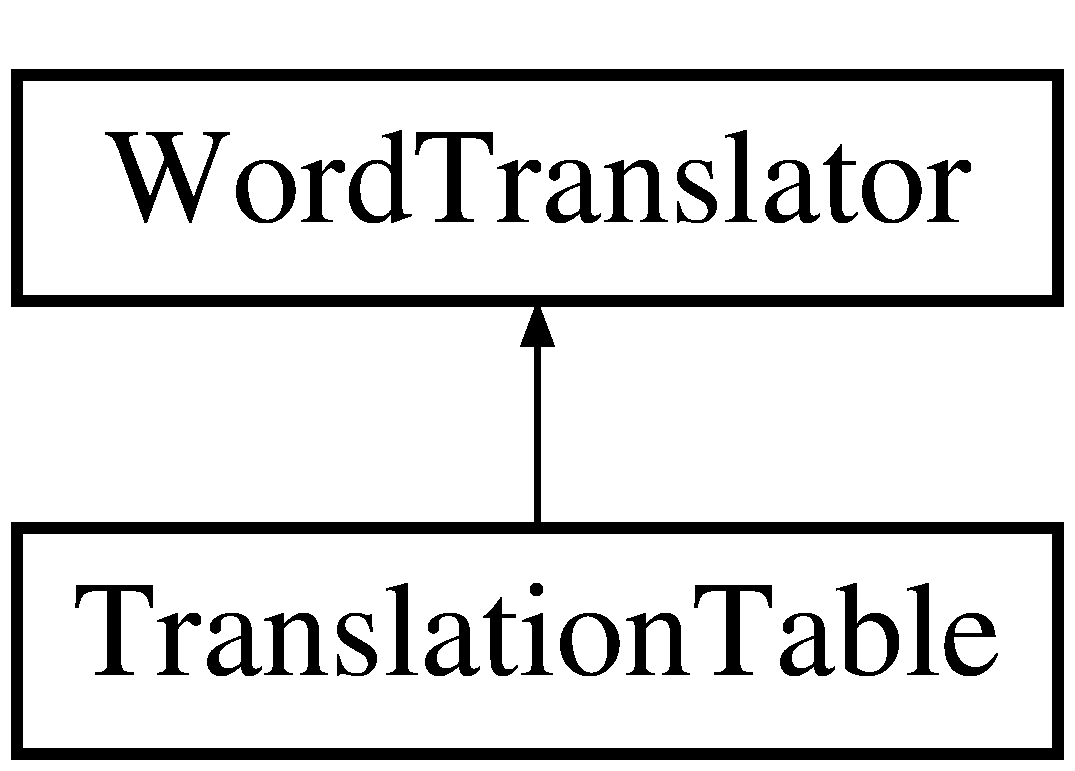
\includegraphics[height=2.000000cm]{classTranslationTable}
\end{center}
\end{figure}
\subsection*{Public Member Functions}
\begin{DoxyCompactItemize}
\item 
\mbox{\Hypertarget{classTranslationTable_a194a18a3efa0ad776e99e73c6a385bca}\label{classTranslationTable_a194a18a3efa0ad776e99e73c6a385bca}} 
void {\bfseries create} (const \hyperlink{classLexicon}{Lexicon} \&correct\+Lexicon, const \hyperlink{classLexicon}{Lexicon} \&incorrect\+Lexicon, \hyperlink{classFile}{File} \&incorrect, \hyperlink{classFile}{File} \&correct)
\item 
\mbox{\Hypertarget{classTranslationTable_a1d06855e760f3d39c57a188b0059e99a}\label{classTranslationTable_a1d06855e760f3d39c57a188b0059e99a}} 
void {\bfseries print} (F\+I\+LE $\ast$output)
\item 
\mbox{\Hypertarget{classTranslationTable_ae8e6848bfd3221e1ba0c9cada67222c6}\label{classTranslationTable_ae8e6848bfd3221e1ba0c9cada67222c6}} 
void {\bfseries print\+For\+Debug} (F\+I\+LE $\ast$output, \hyperlink{classLexicon}{Lexicon} \&correct\+Lex, \hyperlink{classLexicon}{Lexicon} \&incorrect\+Lex)
\item 
\mbox{\Hypertarget{classTranslationTable_a0856b27e0567627e2fc625dbc92a2d7a}\label{classTranslationTable_a0856b27e0567627e2fc625dbc92a2d7a}} 
void {\bfseries read} (\hyperlink{classFile}{File} \&input)
\item 
\mbox{\Hypertarget{classTranslationTable_aa16adfec6d2f059c26460e824d33ed9f}\label{classTranslationTable_aa16adfec6d2f059c26460e824d33ed9f}} 
void {\bfseries add\+Translations} (\hyperlink{classWordTranslations}{Word\+Translations} \&actual)
\end{DoxyCompactItemize}
\subsection*{Additional Inherited Members}


The documentation for this class was generated from the following files\+:\begin{DoxyCompactItemize}
\item 
Translation\+Table.\+hpp\item 
Translation\+Table.\+cpp\end{DoxyCompactItemize}

\hypertarget{classViterbi}{}\section{Viterbi Class Reference}
\label{classViterbi}\index{Viterbi@{Viterbi}}
\subsection*{Public Member Functions}
\begin{DoxyCompactItemize}
\item 
\mbox{\Hypertarget{classViterbi_ae99b04e927af06a69689ad333f6069b5}\label{classViterbi_ae99b04e927af06a69689ad333f6069b5}} 
{\bfseries Viterbi} (\hyperlink{classDatabase}{Database} \&database)
\item 
\mbox{\Hypertarget{classViterbi_ac7b573f62eea989f1abbfbabb0bcdaa0}\label{classViterbi_ac7b573f62eea989f1abbfbabb0bcdaa0}} 
\hyperlink{classFile}{File} $\ast$ {\bfseries correct} (std\+::string input\+Filename)
\end{DoxyCompactItemize}


The documentation for this class was generated from the following files\+:\begin{DoxyCompactItemize}
\item 
Viterbi.\+hpp\item 
Viterbi.\+cpp\end{DoxyCompactItemize}

\hypertarget{classWordTranslations}{}\section{Word\+Translations Class Reference}
\label{classWordTranslations}\index{Word\+Translations@{Word\+Translations}}
\subsection*{Public Types}
\begin{DoxyCompactItemize}
\item 
\mbox{\Hypertarget{classWordTranslations_af5fb38888c5aebb46245a69dc09da445}\label{classWordTranslations_af5fb38888c5aebb46245a69dc09da445}} 
using {\bfseries Pair} = std\+::pair$<$ unsigned int, float $>$
\end{DoxyCompactItemize}
\subsection*{Public Member Functions}
\begin{DoxyCompactItemize}
\item 
\mbox{\Hypertarget{classWordTranslations_ac0f45e5c4155787ca85297cd82df3c6c}\label{classWordTranslations_ac0f45e5c4155787ca85297cd82df3c6c}} 
float {\bfseries combine\+Probas} (float p1, float p2)
\item 
\mbox{\Hypertarget{classWordTranslations_aac43127bc3f117331995c214f94ac92f}\label{classWordTranslations_aac43127bc3f117331995c214f94ac92f}} 
void {\bfseries init\+For\+Token} (unsigned int token)
\item 
\mbox{\Hypertarget{classWordTranslations_aaf8af6a16f9831e622c23eca84608e0f}\label{classWordTranslations_aaf8af6a16f9831e622c23eca84608e0f}} 
void {\bfseries add\+Translation} (unsigned int token, float proba)
\item 
\mbox{\Hypertarget{classWordTranslations_a5e4f3e0e4c51b4aac6a60a3dd16001f7}\label{classWordTranslations_a5e4f3e0e4c51b4aac6a60a3dd16001f7}} 
bool {\bfseries empty} ()
\end{DoxyCompactItemize}
\subsection*{Public Attributes}
\begin{DoxyCompactItemize}
\item 
\mbox{\Hypertarget{classWordTranslations_aa5ab1c43ddab547d46bd4d1e5cb3bfc1}\label{classWordTranslations_aa5ab1c43ddab547d46bd4d1e5cb3bfc1}} 
unsigned int {\bfseries token}
\item 
\mbox{\Hypertarget{classWordTranslations_ab1104aea3c7de7c4e16b529cc6bd371e}\label{classWordTranslations_ab1104aea3c7de7c4e16b529cc6bd371e}} 
std\+::vector$<$ std\+::unique\+\_\+ptr$<$ Pair $>$ $>$ {\bfseries translations}
\item 
\mbox{\Hypertarget{classWordTranslations_a825d6d8ded379c5b19b3fd53d2a2faaa}\label{classWordTranslations_a825d6d8ded379c5b19b3fd53d2a2faaa}} 
std\+::unordered\+\_\+map$<$ unsigned int, Pair $\ast$ $>$ {\bfseries positions}
\end{DoxyCompactItemize}


The documentation for this class was generated from the following files\+:\begin{DoxyCompactItemize}
\item 
Word\+Translator.\+hpp\item 
Word\+Translator.\+cpp\end{DoxyCompactItemize}

\hypertarget{classWordTranslator}{}\section{Word\+Translator Class Reference}
\label{classWordTranslator}\index{Word\+Translator@{Word\+Translator}}
Inheritance diagram for Word\+Translator\+:\begin{figure}[H]
\begin{center}
\leavevmode
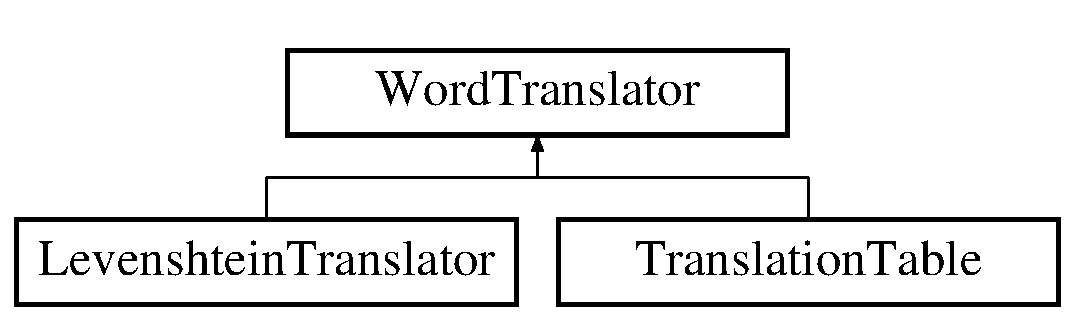
\includegraphics[height=2.000000cm]{classWordTranslator}
\end{center}
\end{figure}
\subsection*{Public Member Functions}
\begin{DoxyCompactItemize}
\item 
\mbox{\Hypertarget{classWordTranslator_a21d741b1316bdf315a4c9346900e1846}\label{classWordTranslator_a21d741b1316bdf315a4c9346900e1846}} 
virtual void {\bfseries add\+Translations} (\hyperlink{classWordTranslations}{Word\+Translations} \&actual)=0
\end{DoxyCompactItemize}
\subsection*{Public Attributes}
\begin{DoxyCompactItemize}
\item 
\mbox{\Hypertarget{classWordTranslator_a179d2bbd6de97dc89397ed0b6322de76}\label{classWordTranslator_a179d2bbd6de97dc89397ed0b6322de76}} 
unsigned int {\bfseries order}
\end{DoxyCompactItemize}


The documentation for this class was generated from the following file\+:\begin{DoxyCompactItemize}
\item 
Word\+Translator.\+hpp\end{DoxyCompactItemize}

\chapter{File Documentation}
\hypertarget{Database_8hpp}{}\section{Database.\+hpp File Reference}
\label{Database_8hpp}\index{Database.\+hpp@{Database.\+hpp}}
{\ttfamily \#include $<$string$>$}\newline
{\ttfamily \#include \char`\"{}Lexicon.\+hpp\char`\"{}}\newline
{\ttfamily \#include \char`\"{}Grams\+Counter.\+hpp\char`\"{}}\newline
{\ttfamily \#include \char`\"{}Translation\+Table.\+hpp\char`\"{}}\newline
{\ttfamily \#include \char`\"{}Levenshtein\+Translator.\+hpp\char`\"{}}\newline
\subsection*{Classes}
\begin{DoxyCompactItemize}
\item 
class \hyperlink{classDatabase}{Database}
\begin{DoxyCompactList}\small\item\em Contains necessary data to perform a correction. \end{DoxyCompactList}\end{DoxyCompactItemize}


\subsection{Detailed Description}
\begin{DoxyAuthor}{Author}
Franck Dary 
\end{DoxyAuthor}

%--- End generated contents ---

% Index
\backmatter
\newpage
\phantomsection
\clearemptydoublepage
\addcontentsline{toc}{chapter}{Index}
\printindex

\end{document}
